\section*{热学B(9.21-9.27)}
\lsn{1}默写与理想气体相关的公式：
\begin{table}[htbp]
  \begin{tabular}{r p{4cm}|rp{4cm}}
    \toprule
    &公式&&公式\\
    \hline
    气体压强&&液体压强&\\
    \hline
    理想气体方程&&克拉珀龙方程&\\
    \hline
    玻意耳定律&&查理定律&\\
    \hline
    盖吕萨克定律&&密度方程&\\
    \hline
    混合气体方程&\multicolumn{3}{c}{}\\
    \bottomrule
  \end{tabular}
\end{table}

\lsn{2}默写热力学三定律：
\vspace*{4cm}

\lsn{3}画出\,\qty{0}{\degreeCelsius}和\,\qty{100}{\degreeCelsius}氧气的分子速率分布曲线：
\vspace*{4cm}

\lsn{4}固体怎样分类，并注明是各向同性还是各向异性：
\vspace*{4cm}

\lsn{5}阐述气体压强产生的机制。

\newpage

\lsn{6}将一根长度 \( L = \) \,\qty{103}{cm} 的长玻璃管竖直放置，管的 \(A\) 端开口，\(B\) 端封闭。利用水银在管的下部封闭着一段空气柱，各段初始长度如图所示。已知外界大气压 \( p_0 = \) \,\qty{76}{cmHg}，温度始终不变。

	\begin{enumerate}
    	\item[(1)] 被封闭的气体压强是多大？
    	\item[(2)] 缓慢将玻璃管绕通过 \(B\) 点的水平轴转动\,\qty{90}{\degree}，使管水平，此时管内空气柱的长度是多长？
	\end{enumerate}

	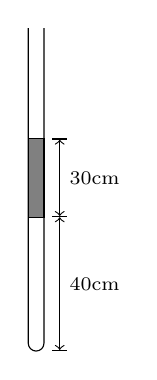
\begin{tikzpicture}
		\draw (0,4)--(0,0) arc(-180:0:.1)--(.2,4);
		\draw[fill=gray] (0,1.6) rectangle(.2,2.6);
		\draw[|<->|] (.4,2.6)--node[right]{\scriptsize \qty{30}{cm}}(.4,1.6);
		\draw[<->|] (.4,1.6)--node[right]{\scriptsize \qty{40}{cm}}(.4,-.1);
	\end{tikzpicture}
\vspace*{1cm}

\lsn{7}如下图所示，将粗细不同的玻璃管插入水和水银中，试画出试管中的液面

\begin{tikzpicture}[font=\footnotesize]
    \draw[fill=gray!30] (0,0) rectangle(4,1.5);
    \draw[very thick] (0,3)--(0,0)--(4,0)--(4,3);
    \draw[fill=white,draw=white] (1.4,.5) rectangle(1.7,1.6) (2.5,.5) rectangle(2.65,1.6);
    \foreach \x in {1.4,1.7,2.5,2.65}
        \draw[very thin] (\x,.5)--(\x,2.8);
    \node at(3.5,.4){水};
    \begin{scope}[xshift=6cm]
        \draw[fill=gray!30] (0,0) rectangle(4,1.5);
        \draw[very thick] (0,3)--(0,0)--(4,0)--(4,3);
        \draw[fill=white,draw=white] (1.4,.5) rectangle(1.7,1.6) (2.5,.5) rectangle(2.65,1.6);
        \foreach \x in {1.4,1.7,2.5,2.65}
            \draw[very thin] (\x,.5)--(\x,2.8);
        \node at(3.5,.4){水银};
    \end{scope}
\end{tikzpicture}

\lsn{8}\lkf{2021 广东，15(2)，6分}
	为方便抽取密封药瓶里的药液，护士一般先用注射器注入少量气体到药瓶里后再抽取药液，如图所示。某种药瓶的容积为\,\qty{0.9}{\ml}，内装有\,\qty{0.5}{\ml}的药液，瓶内气体压强为\,\qty{1.0e5}{Pa}。护士把注射器内横	截面积为\,\qty{0.3}{\cm^2}、长度为\,\qty{0.4}{\cm^2}、压强为\,\qty{1.0e5}{Pa}的气体注入药瓶，若瓶内外温度相同且保持不变，气体视为理想气体，求此时药瓶内气体的压强。

	\begin{tikzpicture}[scale=.8]
		\draw[fill=gray!70] (-.7,-.3) rectangle(-.3,-.7) (-.75,-.7) rectangle(-.25,-.75);
		\draw[fill=gray] (0,0) arc(0:-180:.5)--(-1,1.1)--(0,1.1)--(0,0);
		\draw (0,1.1)--(0,2.2)--(-1,2.2)--(-1,1.1);
		\draw (-.5,-.95)--(-.5,.2);
		\draw (-.6,-1.9) rectangle(-.4,-3.8) (-.65,-1.2) rectangle(-.35,-3) (-.6,-1.2) rectangle(-.4,-1.1) (-.55,-1.1) rectangle(-.45,-.95);
		\draw[fill=white] (-.65,-1.9) rectangle(-.35,-2.1) (-.7,-3) rectangle(-.3,-3.1) (-.75,-3.8) rectangle(-.25,-3.85);
		\draw[pattern=north east lines] (-.65,-1.9) rectangle(-.35,-2.1);
	\end{tikzpicture}

\newpage
\lsn{9}在如图所示的坐标系中，一定质量的某种理想气体先后发生以下两种状态变化过程：第一种变化是从状态\(A\)到状态\(B\)，外界对该气体做功为\,\qty{6}{J}；第二种变化是从状态\(A\)到	状态\(C\)，该气体从外界吸收的热量为\,\qty{9}{J}。图	线\(AC\)的反向延长线过坐标原点\(O\)，\(B\)、\(C\)两状态的温度相同，理想气体的分子势能为零。求：
	\begin{enumerate}
		\item[(1)] 从状态\(A\)到状态\(C\)的过程，该气体对外界做的功\(W_1\)和其内能的增量\(\Delta U_1\)；
		\item[(2)] 从状态\(A\)到状态\(B\)的过程，该气体内能的增量\(\Delta U_2\)及其从外界吸收的热量\(Q_2\)。
	\end{enumerate}
    \begin{tikzpicture}[>=stealth,font=\scriptsize]
        \draw[blue,->] (0,0)--(4,0)node[below]{\(T\)};
        \draw[blue,->] (0,0)node[below left]{\(O\)}--(0,3)node[right]{\(p\)};
        \draw[dashed] (0,0)--(1.5,.7)node[above left,red]{\(A\)} (1.5,.7)--(1.5,0)node[below,blue]{\(T_1\)} (3,2.8)--(3,0)node[below,blue]{\(T_2\)};
        \draw[->,purple] (1.5,.7)--(3,1.4)node[right]{\(B\)};
        \draw[->,purple] (1.5,.7)--(3,2.5)node[right]{\(C\)};
    \end{tikzpicture}

\lsn{10}写出“用油膜法估算油酸分子的大小”实验原理、实验器材、实验步骤。
\vspace*{11cm}

\lsn{11}写出下列情景中对油酸分直径测量的影响并分析误差成因

\begin{table}[htbp]
    \begin{tabular}{r|c|p{8cm}}
        \hline
        情景&误差大小&误差原因\\
        \hline
        撒粉太多太厚&&\\
        \hline
        没有充分静置&&\\
        \hline
        滴数多数&&\\
        \hline
        不完整方格当作完整&&\\
        \hline
        溶液长时间放置&&\\
        \hline
    \end{tabular}
\end{table}